%!TEX encoding = IsoLatin

%
% Chapitre "Objectifs"
%

\chapter{Besoins et objectifs}
\label{s:objectifs}

\section{Analyse des besoins}

Afin de bien saisir la demande du client et de lui fournir une solution appropriée, une analyse des besoins sera réalisée. 

\subsection{Capteur optique autonome}

Pour commencer, l'automatisation et l'autonomie seront au coeur de ce projet. Le design doit comprendre un capteur optique qui recueillera des images des poissons observés. Le capteur optique doit être en mesure de prendre des photos en couleur sans interventions humaines. Ainsi, le capteur doit être muni d'un dispositif de détection de mouvement. Les images prise suite à l'identification doivent également être envoyées avec certaines informations physiques, dont la date et l'heure, la température interne du système ainsi que la température de l'eau lors de la prise de la photo. Le capteur optique doit être fonctionnel pour une durée minimale de deux semaines avant d'avoir recours à une maintenance. De plus, le capteur se doit d'être opérationnel en tout temps. Or, la caméra utilisée devra être d'une qualité suffisante pour permettre la reconnaissance du poisson, et ce, même la nuit.

\subsection{Système d'identification des poissons}

Le système d'identification des poissons est l'un des principaux besoins du client. En effet, le client souhaite recueillir des statistiques et une certaine documentation sur la faune aquatique. Pour y arriver, le système doit être en mesure d'identifier et de comptabiliser un minimum de cinq espèces de poissons évoluant dans un milieu aquatique à partir d'une prise de mesure non invasive. Comme mentionné précédemment, il est nécessaire d'assurer l'automatisation de l'identification des poissons.

%Le système se devra donc d'avoir un dispositif lui permettant de savoir quand prendre des photos et savoir si la photo contient bel et bien un poisson. L'enregistrement des données doit aussi se faire automatiquement. Après la collecte de données, le système sera tenu de stocker les données par lui-même pour une durée minimale de deux ans. Ensuite, il faudra gérer l'identification des poissons. Pour que le système soit efficace, il devra être en mesure d'identifier jusqu'à cinq variétés de poissons différentes, et ce, sans intervention humaine. Dans la même lancée, le système devra être autonome pour effectuer ces fonctions. 

\subsection{Interaction et sécurité du système}

L'interaction avec le système est primordiale afin de gérer les données du système et de recueillir les statistiques désirées. Le système doit permettre à l'usager de configurer et d'assurer les opérations du capteur à distance. Plus concrètement, l'utilisateur devra être capable d'avoir accès aux données en tout temps, et ce, peu importe sa localisation. Un serveur doit donc être implémenté pour permettre à l'usager de communiquer au capteur et ses archives sous une connexion sécurisée. En effet, par souci de confidentialité des renseignements et des données, toutes les connexions devront être sécurisées. Seul un utilisateur ayant une autorisation pourra communiquer avec le système. L'opérateur du capteur doit également pouvoir interagir avec le capteur à l'aide d'une interface locale.

Afin d'assurer la sécurité, le système doit être capable de générer des alarmes. Celles-ci seront acheminées vers l'opérateur du système en cas de défaillance de certaines fonctionnalités. 

\subsection{Archives des données}

Afin de collecter les informations et les statistiques du site aquatique, le système doit être muni d'un dispositif d'entreposage des données. Les archives devront comprendre certains éléments. D'abord, suite à l'identification des poissons, les images originales doivent être stockées dans le système à des fins de traitements et de validation ultérieur. Elles devront également être stockée avec leur vignette, soit les conditions enregistrées lors de la prise de la photo. De plus, les alarmes, les paramètres de configuration et les commentaires relevés par le responsable du capteur devront être archivés. L'ensemble de ces informations doivent être entreposées et accessibles pour une durée de deux ans.

\newpage{}

\section{Objectifs}

\begin{enumerate}

    \item Assurer un produit de qualité
    \begin{itemize}
        \item Maximiser la durée de vie de l'appareil
        \item Maximiser la précision et l'exactitude du logiciel de reconnaissance 
        \item Optimiser l'utilisation de l'interface graphique
        \item Maximiser les variétés de poissons identifiables
        \item Maximiser la capacité de stockage des données
        \item Maximiser la fiabilité du système de sécurité
    \end{itemize}
    
    \item Assurer le respect des contraintes
    \begin{itemize}
        \item Assurer une mesure passive du système
        \item Assurer le respect des contraintes mécaniques en milieu marin
        \item Assurer le respect des contraintes reliées aux images
    \end{itemize}

    \item Minimiser l'intervention humaine
    \begin{itemize}
        \item Maximiser la durée de vie de la batterie
        \item Minimiser la complexité de la maintenance
        \item Maximiser l'automatisation du transfert des données
        \item Faciliter l'accès à distance
    \end{itemize}
    
    \item Maximiser la facilité de conception
    \begin{itemize}
        \item Minimiser le temps de conception du produit
        \item Minimiser la complexité de l'usinage des pièces
        \item Faciliter la rechange des pièces
        \item Faciliter l'implantation du capteur sur différents sites
    \end{itemize}
    
    \item Minimiser les coûts
    \begin{itemize}
        \item Minimiser les coûts de conception du produit
        \item Minimiser les frais d'installation
        \item Minimiser les frais de maintenance et d'opération
        \item Minimiser le coût de remplacement des pièces
        \item Respecter les contraintes lié coûts globaux
    \end{itemize}
    
    \newpage
    
    \begin{figure}
        \centering
        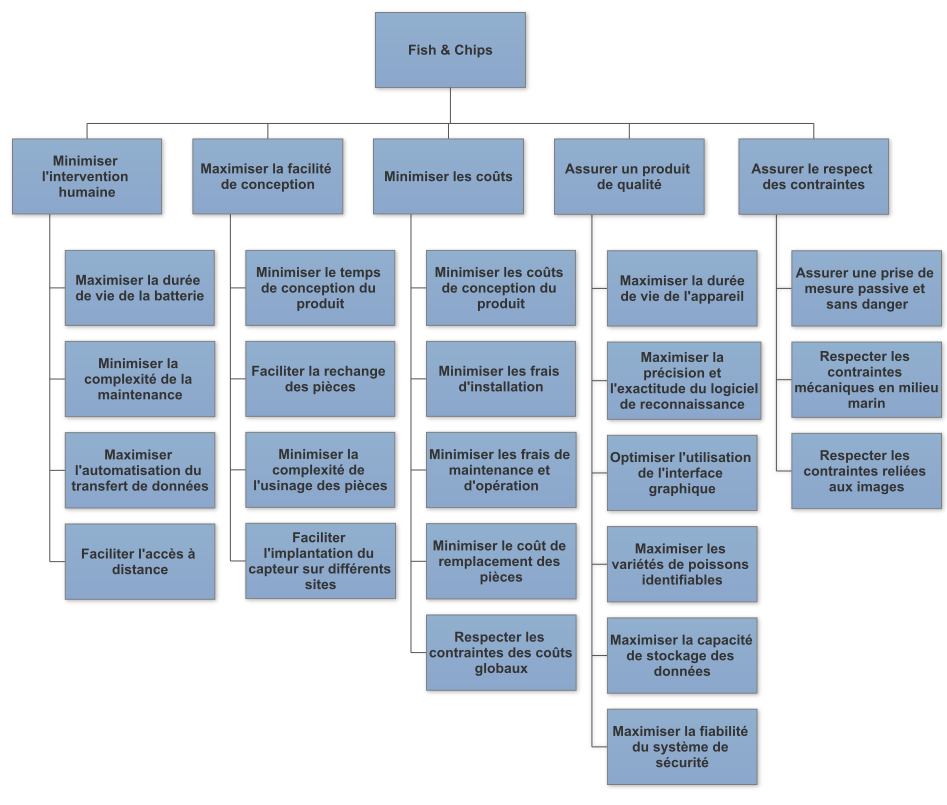
\includegraphics[width=1.0\linewidth]{fig/Organigramme.png}
        \caption{Organigramme des objectifs du projet Fish \& Chips}
        \label{fig:organigramme}
    \end{figure}
    
    %\item Autres (je sais pas dans quelle catégorie les mettre)
    %\begin{itemize}
    %    \item Maximiser la disponibilité du capteur
    %    \item Maximiser la sécurité
    %    \item Assurer une mesure passive
    %\end{itemize}
    
\end{enumerate}
